
%%%%%%%%%%%%%%%%%%%%%%% file typeinst.tex %%%%%%%%%%%%%%%%%%%%%%%%%
%
% This is the LaTeX source for the instructions to authors using
% the LaTeX document class 'llncs.cls' for contributions to
% the Lecture Notes in Computer Sciences series.
% http://www.springer.com/lncs       Springer Heidelberg 2006/05/04
%
% It may be used as a template for your own input - copy it
% to a new file with a new name and use it as the basis
% for your article.
%
% NB: the document class 'llncs' has its own and detailed documentation, see
% ftp://ftp.springer.de/data/pubftp/pub/tex/latex/llncs/latex2e/llncsdoc.pdf
%
%%%%%%%%%%%%%%%%%%%%%%%%%%%%%%%%%%%%%%%%%%%%%%%%%%%%%%%%%%%%%%%%%%%

% ○ 問題を沢山使ってる例を出す
% わからない問題でもいいことを示す Who's the bully? when?
% ○エピソードを使う認証は多いが、パスワードを生成するものは何故かない
% ○  毎日の行動から認証するものもある
% 家族や友人が知らない秘密は存在するはず
% 秘密の質問が駄目と言われるのは質問の質が悪いから
%
% ○ 拡張機能の説明
%
% ○ 参考文献たくさん
% 大きなことをいわない
% パスワードを覚えるのは無理
% ○ シード文字列の選びかた
% エントロピーの計算
% アルゴリズムの選択 
% 偽答生成が簡単であることを示す 
% サポートシステムを作っていることをかく ★

\documentclass[runningheads,a4paper]{llncs}

\usepackage{amssymb}
\setcounter{tocdepth}{3}
\usepackage{graphicx}

\usepackage{here} % [H]とするとその場所に配置されるらしい

\usepackage{url}
\urldef{\mailsa}\path|masui@pitecan.com|
\newcommand{\keywords}[1]{\par\addvspace\baselineskip
\noindent\keywordname\enspace\ignorespaces#1}

\begin{document}

\mainmatter  % start of an individual contribution

% first the title is needed
\title{EpisoPass: Password Management based on Episodic Memories}

% a short form should be given in case it is too long for the running head
\titlerunning{Lecture Notes in Computer Science: Authors' Instructions}

% the name(s) of the author(s) follow(s) next
%
% NB: Chinese authors should write their first names(s) in front of
% their surnames. This ensures that the names appear correctly in
% the running heads and the author index.
%
\author{Toshiyuki Masui%
\thanks{Thanks...}%
}
%
\authorrunning{Lecture Notes in Computer Science: Authors' Instructions}
% (feature abused for this document to repeat the title also on left hand pages)

% the affiliations are given next; don't give your e-mail address
% unless you accept that it will be published
\institute{Faculty of Environment and Information Studies, Keio University\\
5322 Endo, Fujisawa, Kanagawa 252-8520, Japan\\
\mailsa\\
\url{http://pitecan.com/}}

%
% NB: a more complex sample for affiliations and the mapping to the
% corresponding authors can be found in the file "llncs.dem"
% (search for the string "\mainmatter" where a contribution starts).
% "llncs.dem" accompanies the document class "llncs.cls".
%

\toctitle{Lecture Notes in Computer Science}
\tocauthor{Authors' Instructions}
\maketitle


\begin{abstract}
We propose a password manager \textit{EpisoPass} that supports the
generation of strong passwords based on a user's secret episodic
memories. To use EpisoPass, a user first collects question-answer
pairs related to their own episodic memories. Each is registered with
several possible answers: a single correct answer and multiple fake
answers. When the user wants to generate a password, EpisoPass shows
each question and list of possible answers and asks the user to select
those that are correct. EpisoPass then generates a domain-unique
password by substituting the characters of a seed string based on the
selected answers. Through careful selection of memories and answers,
EpisoPass provides an authentication step using memories that are easy
to recall, but difficult for others to guess. In this way various
strong passwords can be easily managed without the need for the master
password or secret device that is otherwise required by conventional
password managers. Using a browser extension, users can use EpisoPass
directly on the login page of conventional Web services like Facebook,
removing the need to type or copy a password string.

\keywords{Passwords; password managers; user authentication; episodic memories; EpisoPass}
\end{abstract}

\section{Introduction}

Passwords have been used for various Web services and applications
for a long time, and currently the most popular authentication method on the Internet.
%
Since short passwords are easily guessed by attackers and
using the same password for different services is unsafe,
different long passwords should be used for different services.
However,
remembering many long passwords is almost impossible for ordinary humans.
%
According to a research in 2007,
people use 6.5 passwords on 25 Web services on average, and
4.28\% of the users forget their passwords in 3 months\cite{Florencio:2007:LSW:1242572.1242661}.

Since passwords are difficult to handle,
various other authentication methods have been proposed.
For example,
image-based authentication\cite{Biddle:2012:GPL:2333112.2333114}\cite{GraphicalPasswords}, 
biometrics authentication\footnote{
  % \textsf{https:{\slash}{\slash}en.wikipedia.org{\slash}wiki{\slash}Biometrics}
  \url{https://en.wikipedia.org/wiki/Biometrics}
},
behavior-based authentication\cite{Dandapat:2015:AYD:2702123.2702457}, 
and many other authentication methods have been proposed.

% というのもパスワードには利点があるから[Bonneau]
%   すでに普及
%   KB以外の特殊ハードが要らない
%   アタック方法はいろいろあるし[] 流出もしばしばだが
%     うまく実装したシステム上でうまく使えば安全
%     ハッシュ、ソルト
%     実装が比較的簡単
% なのでパスワードが近い将来死滅するとは考えられない

However,
password-based authentication is still the most
convenient and strong method\cite{Bonneau:ReplacePasswords},
and it is not supposed to become extinct
in a short period of time\cite{Herley:2009:PSS:1601990.1602010}.

If we have to live with password-based authentication systems,
we have to devise some ways to handle many passwords, and
various ``password managers'' have been proposed
\cite{OnePassword}%
\cite{Dashlane}%
\cite{MilPass}%
\cite{LastPass}%
\cite{KeyPass}%
\cite{NortonIDSafe}%
\cite{IDManager}.
%
Password managers remember users' passwords and help them enter
passwords on various services.
%
Most password managers can manage various passwords by
asking users to remember a single ``master password'' to access the database.
%
Although password managers are useful,
users have to remember the master password
or use a special hardware device
for safely handling password managers, and
password managers usually run on limited devices.

% 読みとることができない脳内情報を利用するという基本手法は良いのだが覚えられないのが問題である
%   だとすると...パスワードを記憶するかわりに、****脳が既に覚えている秘密の記憶からパスワードを生成すればよいはずである***
%   確かな脳内情報を使ってパスワードを利用する必要があるが、
%     沢山の強力なパスワードそのものを覚えることは不可能に近い
%   だとすると、確かな脳内秘密情報からパスワードをGenerateするしかない
%   そこでエピソード記憶を使う
%   秘密の知識からGenerateするとよい
%

If we don't want to carry any special device for authentication,
all the information required for the authentication should be
kept in the brain.
%
However, the biggest problem of brain-based authentication is that
users cannot safely keep memories like long passwords or master password.
For this reason, we believe that
it is far better to ``generate'' something for the authentication,
based on users' episodic memories that they can never forget.
%
% We believe that a password manager should have the following features.
% (1) It should be available on any platform including PCs, smartphones, and the Web.
% (2) Users should not have secret information (e.g. master password) or special device.
% (3) Rely only on the information in the user's brain.
%
We propose a password manager \textit{EpisoPass} that generates strong passwords
based only on the user's secret episodic memories that the user cannot forget.

\section{EpisoPass}

EpisoPass is a password manager that supports generating
strong passwords based on users' secret episodic memories.
%
% Before using EpisoPass for generating passwords,
% a user provides a seed string and many question-answer pairs to EpisoPass,
% and a password is generated based on the user's selections.
%
% Memories in human brain are not uniform.
We keep various memories in our brain, but different memories have different natures.
Some memories are very short-lived, and others are unforgettable.
When we have a very impressive experience,
that memory will stay in the brain for a long time and
cannot easily disappear.
On the other hand, when we study math and try to remember a new formula,
it is usually hard to memorize it unless we practice a lot,
since the knowledge about the formula is not related to
any personal experiences.
The former type of memory is called the episodic memory and
people cannot easily lose it.
Memories of passwords belong to the latter type and
people cannot easily remember them, just like people cannot
remember math formulas easily.

% \begin{quote}
% Episodic memory is the memory of autobiographical events (times,
% places, associated emotions, and other contextual who, what, when,
% where, why knowledge) that can be explicitly stated. It is the
% collection of past personal experiences that occurred at a particular
% time and place. For example, if one remembers the party on his or her
% 6th birthday, this is an episodic memory. They allow an individual to
% figuratively travel back in time to remember the event that took place
% at that particular time and place.[1]
% 
% Semantic memory is one of the two types of declarative or explicit
% memory (our memory of facts or events that is explicitly stored and
% retrieved).[1] Semantic memory refers to general world knowledge that
% we have accumulated throughout our lives.[2] This general knowledge
% (facts, ideas, meaning and concepts) is intertwined in experience and
% dependent on culture. Semantic memory is distinct from episodic
% memory, which is our memory of experiences and specific events that
% occur during our lives, from which we can recreate at any given
% point.[3] For instance, semantic memory might contain information
% about what a cat is, whereas episodic memory might contain a specific
% memory of petting a particular cat. We can learn about new concepts by
% applying our knowledge learned from things in the past.[4] The
% counterpart to declarative, or explicit memory, is procedural memory,
% or implicit memory.[5]
% \end{quote}

The idea of using episodic memories for authentication has a long history.
Early papers suggested using episodic memories for creating passwords, and
authentication by using secret questions,
sometimes called as ``cognitive passwords''\cite{Zviran:1990:UAC:100512.100538},
has long been used as an
alternative to password-based authentication systems.
%
However, conversion from episodic memories to password strings
was not studied at all.

Password generation on EpisoPass is performed through the following steps:

\begin{enumerate}
\item A user registers many question texts related to the user's personal
secret episodic memories that the user never forgets,
and provides a correct answer and additional fake answers.

\item The user provides a long ``seed string'' for each service that requires
a password.

\item EpisoPass shows the data to the user so that
the user can select the right answer for each question.
Based on the user's selections,
EpisoPass substitutes characters in the seed string and generates
strong password candidate strings.
After selecting all the right answers,
the user copies the calculated string
and register it as the password for the service.
\end{enumerate}

\subsection{Using EpisoPass on a browser}

Figure \ref{web1} shows how to generate a password
on EpisoPass running on a browser.
Many questions related to the user's episodic memories are shown to the user,
and many candidate answers are also shown for each question.
When a user clicks and selects one of the answers for each question,
the seed string shown at the top-left is converted to a
candidate password string based on the selections.
When the user selects the right answers to all the questions,
the right password is calculated and shown at the top.

% If the q-a is based on the user's episodic memories and
% nobody knows the correct answer,
% only the user can select the set of right answers and
% use the converted string as the password.

\begin{figure}[H]
\centering
% 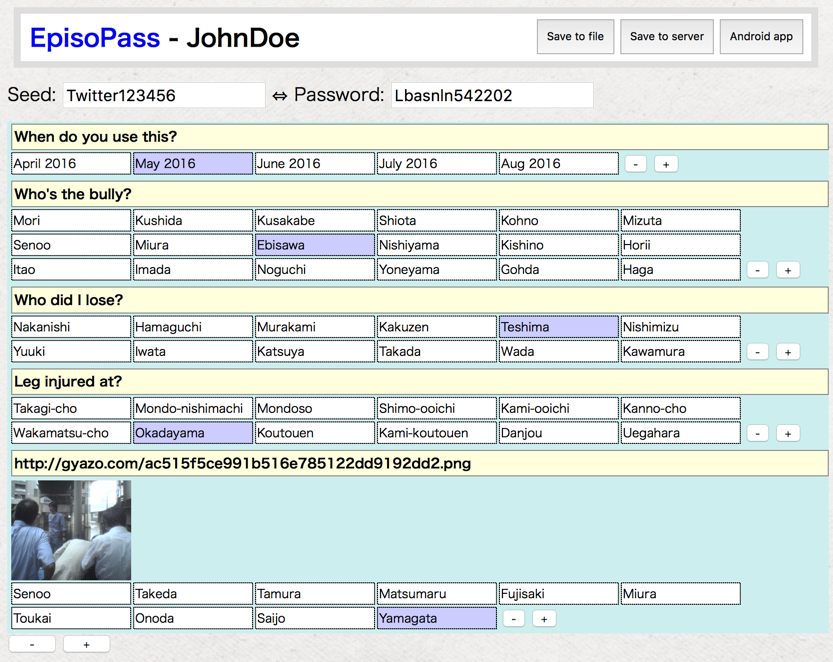
\includegraphics[width=1.0\columnwidth]{figures/c1bd6e7f67698c70978f528ccd2339d9}
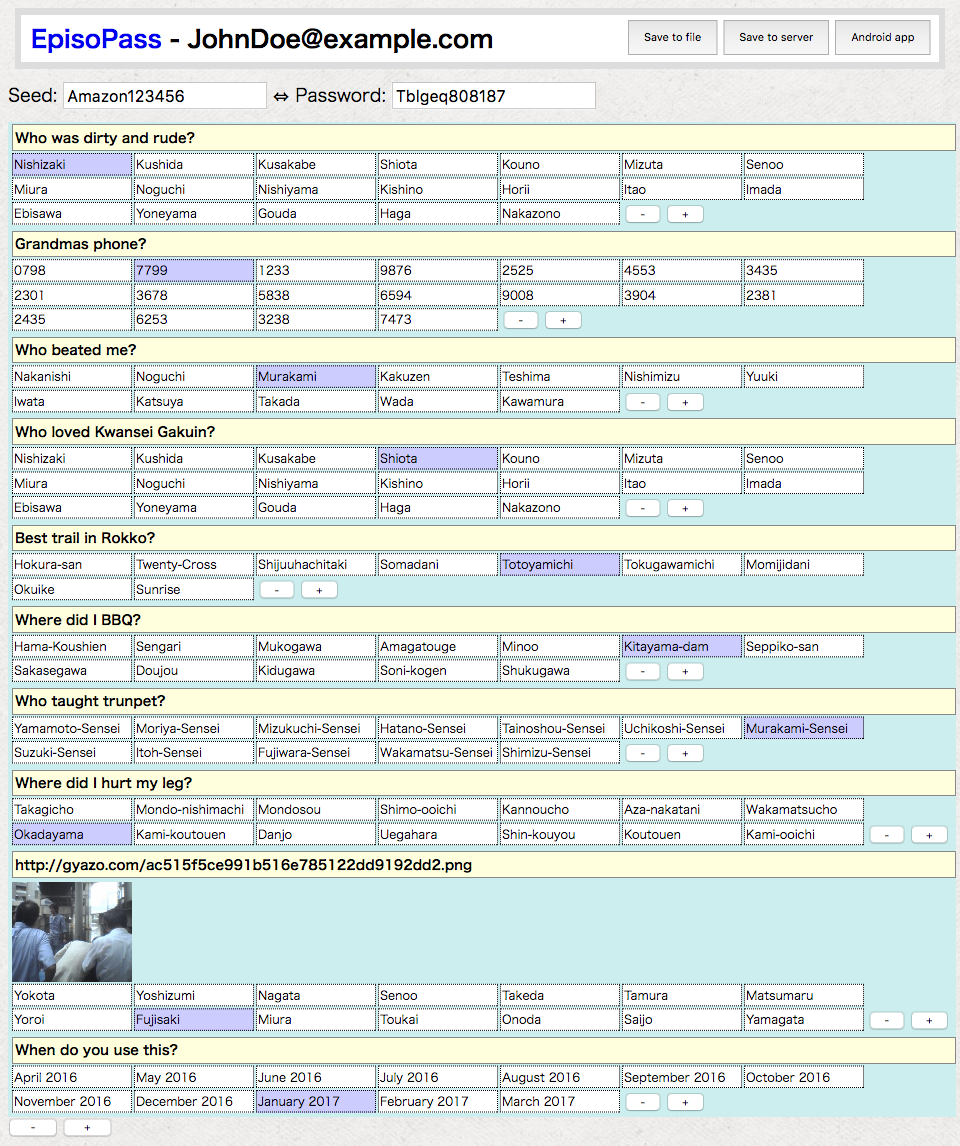
\includegraphics[width=1.0\columnwidth]{figures/4d13e6804ba790624c1f8e2b8255bde5}
\caption{Generating an Amazon password with EpisoPass.}
\label{web1}
\end{figure}

In Figure \ref{web1},
``\textsf{Amazon123456}'' is provided as the seed string,
and according to the selections to the five questions,
the seed string is converted to a string
``\textsf{Tblgeq808187}'',
which can be used as the password for Amazon.com.

When the user clicks another candidate,
the seed string is converted to another strings like
``\textsf{Xvdkzb940345}'' (Figure \ref{web11}).

\begin{figure}[H]
\centering
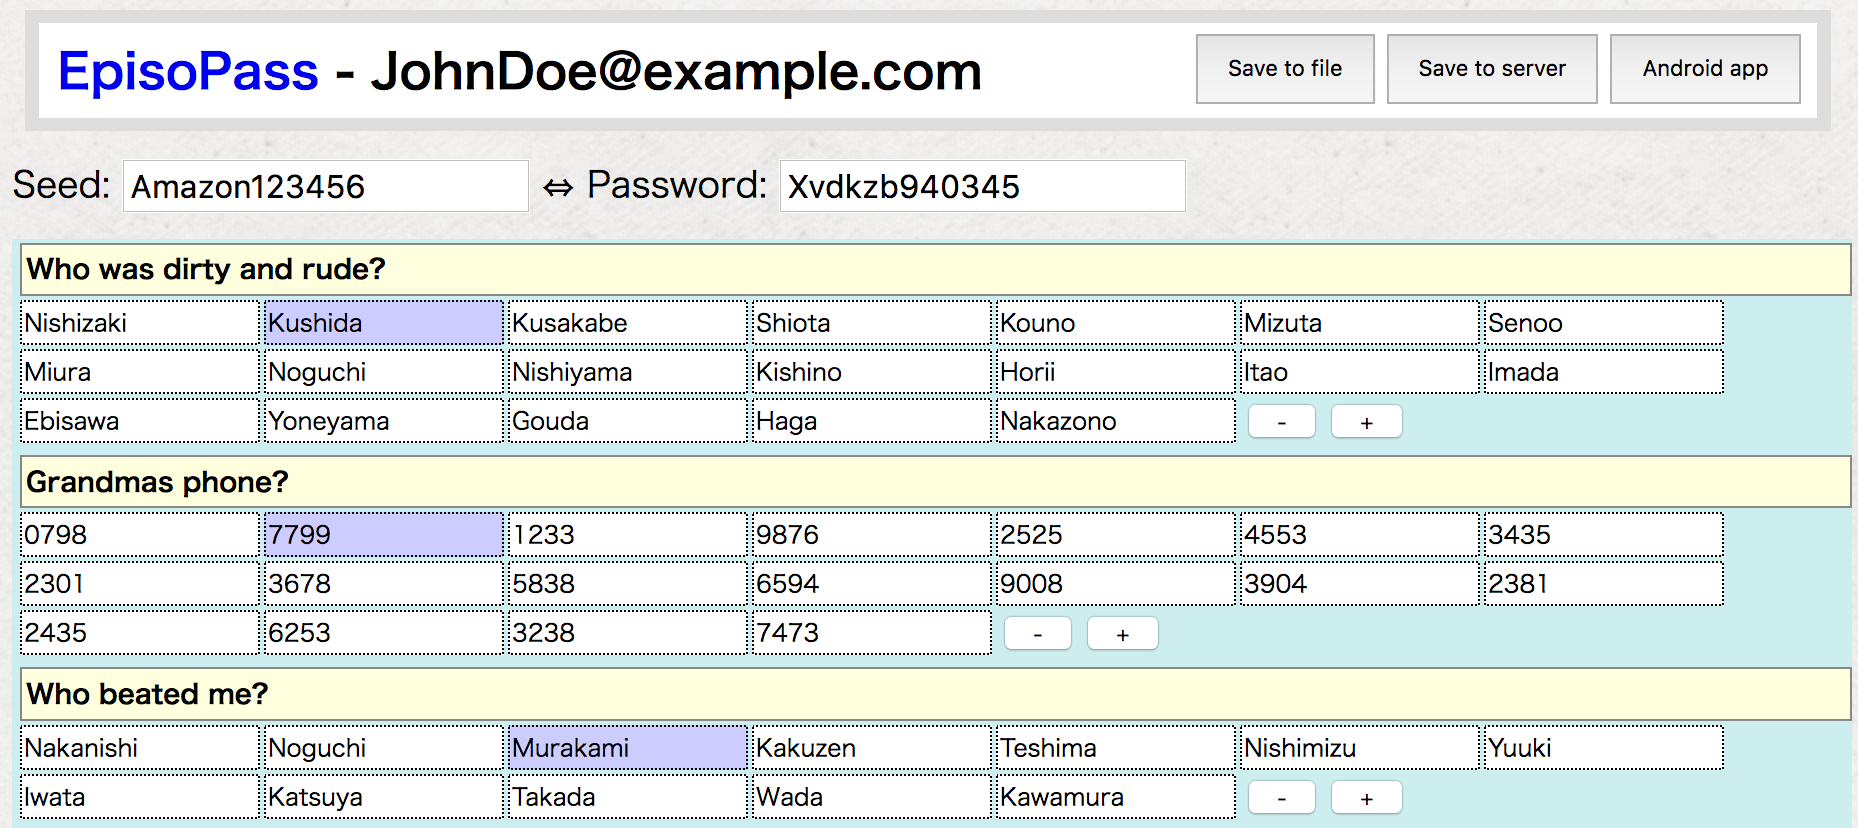
\includegraphics[width=1.0\columnwidth]{figures/8447eaba1ede0f678b3ce6fea63681f3}
\caption{Selecting a different answer.}
\label{web11}
\end{figure}

In this way, different selections yields different password strings and
the password string generated after selecting correct answers can be
used as the password for the service.

Capital letters in the seed string are substituted to capital letters in the password,
and digits in the seed string are substituted to digits,
so that generated passwords conforms to password character restrictions
sometimes requested by the service.

The first question in Figure \ref{web1}
is based on the author's episodic memory at elementary school,
and the question with a photo at the bottom is related to a more recent event
which the author believes he will never forget.
All the questions are based on the author's episodic memories
that he thinks he never forgets, and he believes that
nobody else knows which one of the candidate is the right answer.

Questions and answers can be edited directly on the browser, and they can be
saved on the server by clicking the ``save to server'' button.
The Q-A data sets are saved on the server,
but no information about the correct answer or the
generated password is saved on the server.
The Q-A data in JSON format can be downloaded to the local machine
by cliking the ``save to file'' button.
the data can be uploaded to the server by dragging the JSON file to the EpisoPass page.

When we change the secret string to ``\textsf{Facebook123456}'',
the generated password changes to ``\textsf{Onjbrppy030937}'',
as shown in Figure \ref{web2}.
In this way, we can generate different passwords for
different services just by changing the seed string.

\begin{figure}[H]
  \centering
%  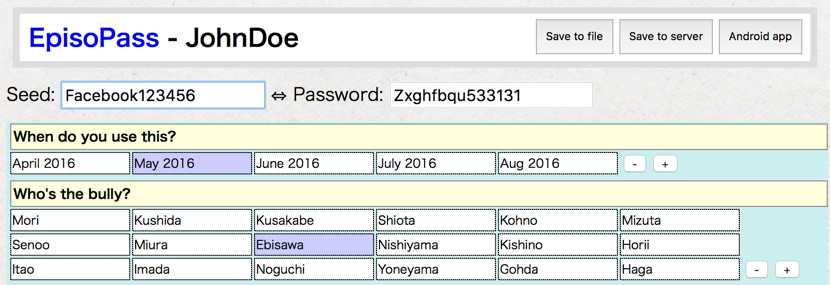
\includegraphics[width=1.0\columnwidth]{figures/0e2820c279afc70520482e0fc53b6ed9}
  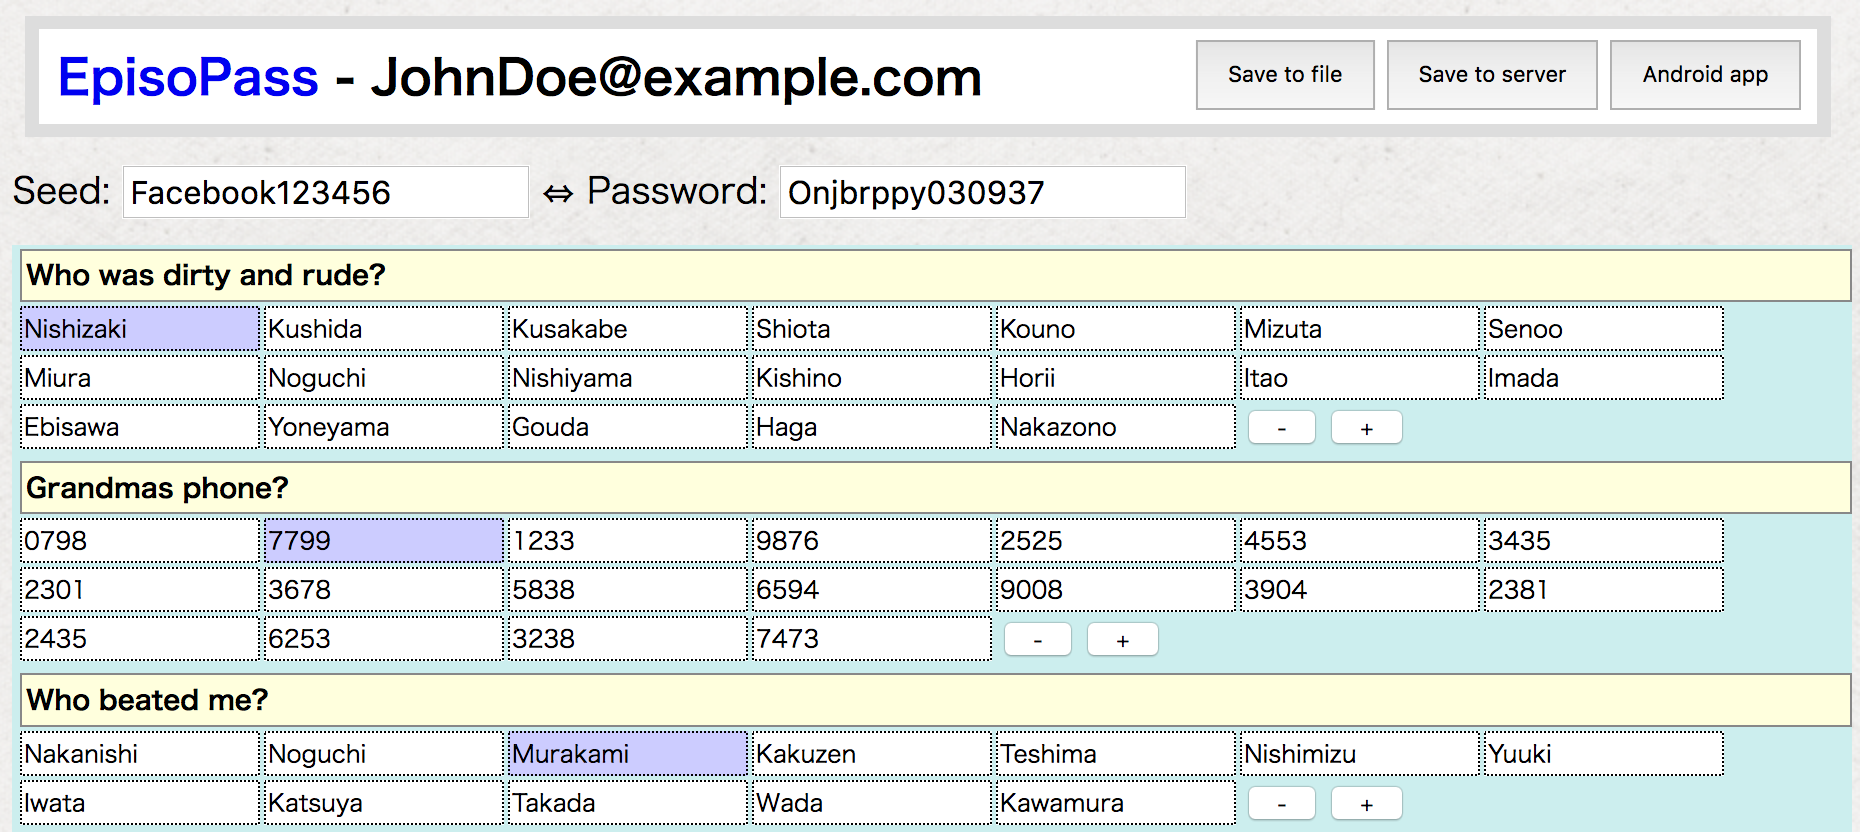
\includegraphics[width=1.0\columnwidth]{figures/ab4517dd593c1cabab5fecef546f7e88}
  \caption{Generating the password for Facebook.}
  \label{web2}
\end{figure}

Character substitution is performed based on the hash value
calculated from concatinating all the selected answers.
%
For example, if the user selects ``\textbf{\texttt{Ebisawa}}'' to the question ``\textbf{\texttt{Who's the bully?}}'',
a hash value calculated from  ``\textbf{\texttt{Who's the bully:Ebisawa}}''
is used for the substitution.

The last question in Figure \ref{web1} is not a secret question, but a question
for generating different passwords for different situations.
By providing such a question, users can generate completely different passwords
for different months and years, for example.

\subsection{Android application}

If a user doesn't like to use EpisoPass service on the Net,
he can use an EpisoPass application on Android
which does not use network connections.
After registering questions and answers on the EpisoPass service,
the user can download an Android application from the server
by clicking the ``Android app'' button at the top.
The application contains all the information required for generating passwords.
(The application is compiled and built on the server.)

When the user runs the application and selects the correct answer
to each question, he can eventually get the password and copy it to the password entry.
(Figure \ref{android1},\ref{android2})

\begin{figure}[H]
\centering
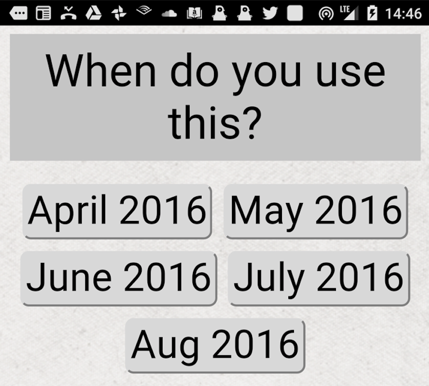
\includegraphics[width=0.7\columnwidth]{figures/429eec261024dc6c85351f51c12f09b4}
\caption{Running EpisoPass on Android.}
\label{android1}
\end{figure}

\begin{figure}[H]
\centering
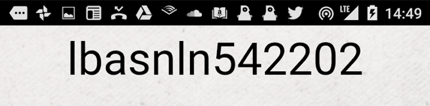
\includegraphics[width=0.7\columnwidth]{figures/ba8f5aeaa935ad63437969f4d746746b}
\caption{After finishing selections.}
\label{android2}
\end{figure}

The calculation is performed on Android without network connection,
and the user can safely generate passwords 
without feeling the fear of being observed by attackers

\subsection{Using the browser extension}

When a user use the EpisoPass service or the EpisoPass application,
he has to type or copy the password string after generating the password.
Since it is not convenient,
we provide a browser extension for using EpisoPass on the login window of
various Web services.


A browser extension is a JavaScript add-on program which runs
on top of existing HTML and JavaScript.
%
Figure \ref{extension} shows the login page of Amazon.com, with which
EpisoPass questions are automatically displayed by the browser extension.
%
Here, when the Amazon login page is accessed from the browser,
the browser extension program automatically runs on the page,
acquires questions and answers from the EpisoPass server,
and shows them to the user just the same way as the Android application.
%
After answering all the questions, a password is calculated from the
selected answers and pasted to the password input form of the page.
Using the extension, users can login to various services just by
answering questions, without seeing any password string.
It looks as if these services are offering
EpisoPass-based authentication.

\begin{figure}[H]
\centering
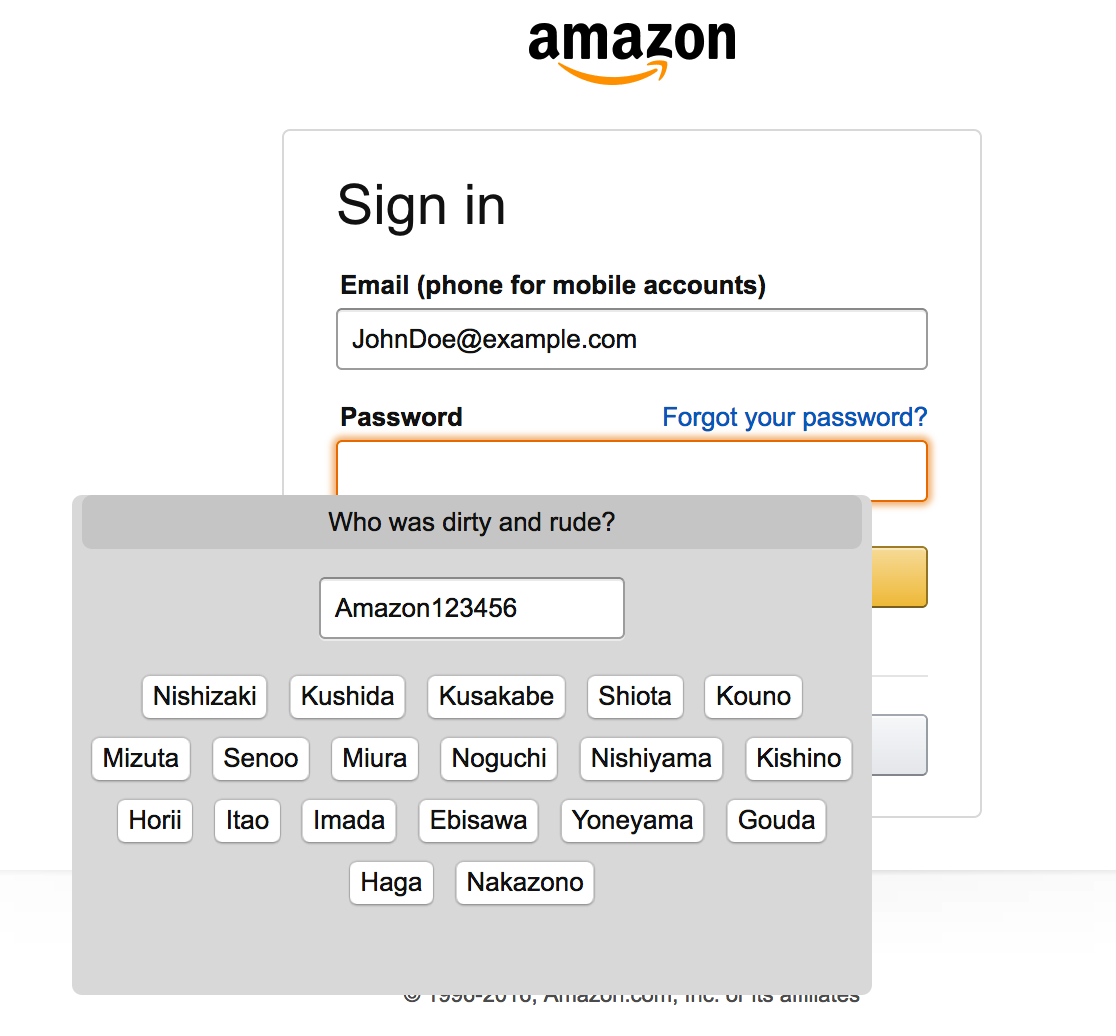
\includegraphics[width=0.9\columnwidth]{figures/aeff16ffcab956e554364e9e5aca8359}
\caption{Using EpisoPass on the login window.}
\label{extension}
\end{figure}

\section{Discussions}

In this section, we discuss the advantages and caveats of using EpisoPass.

\subsection{Recallability of answers}

The biggest advantage of using EpisoPass is that
users don't have to remember strong password strings.
%
Users of EpisoPass can save the seed string and question-answer data
at any place, and easily generate passwords by running
EpisoPass and answering questions.
If the question is based on old unforgettable episodic memories,
there is little chance of losing passwords
as long as the seed string and the questions are available.
If the user's memory is related to an episode of 20 years ago and the user clearly
remembers the episode now, it is unlikely that he forgets the episode 10 years later.

\subsection{Selection of seed strings}

In the previous examples showing the author's real EpisoPass questions,
a seed string ``\textsf{Amazon123456}'' was used for Amazon.com, and
``\textsf{Facebook123456}'' was used for Facebook.
Such strings are used because they are easily memorable.
Of course any seed string can be used as seeds for various services,
and automatic generation of seed strings is possible,
although generating service specific unique seed string is not trivial.
For example, users can use the same username and password both
for Amazon.com and Amazon.co.uk, but not for Amazon.co.jp.

\subsection{Security strength of EpisoPass}

The strength of the generated password depends on the number of
questions and the secret level of the questions.
%
There have been many studies on the strength of passwords
\cite{Hayashi:2011:DSP:1978942.1979326}%
\cite{Komanduri:2011:PPM:1978942.1979321}, % What password is strong
but the strength of secret questions has not been studied enough.
%
When we use 10 secret questions with 20 answers and
there's no clue for the answer,
1 billion ($20^{10}$) trials should be performed to check
all the combinations of the answers,
and the entropy of the system is 43.2 ($10 \times \log_2 20$) bits.  % 10.0 * (Math.log(20.0)/Math.log(2.0))
%
It is almost the same entropy as using random 8-character English alphabets
as a password, in which case the entropy is 45.6 bits.
This level is considered to be strong enough for Web services,
where online brute-force attack is impossible\cite{Florencio:2007:SWP:1361419.1361429}.

\subsection{Selecting good questions}

The quality of the questions is the key to using EpisoPass.
If the episode is shared by someone else,
that person can easily answer the question and generate the
password just like the user.
%
The episode related to each question should not be known to other people,
and the episode should be unforgettable.
%
Finding such episodes seems difficult at first, but
when we try to remember experiences of old days,
we can recall many trivial episodes which are unforgettable but
not important to other people.
%
Old experiences like the following are candidates for
good questions used in EpisoPass.

\begin{itemize}
\item Memory of small injury. (Nobody cares it but you.)

\item Memories of bad experience like blunders or defeat.
(You don't tell it to anybody.)

\item Experience of finding a small special item which only you are interested in.
\end{itemize}

For example, a question like
``who hit you when you were 6 years old?''
is about a trivial experience that people do not mention,
but a bad experience like this is not forgettable.

Questions like ``Which food do you like best?'' should be avoided,
since some of the friends might know the user's taste.
Questions related to an episode which the user is proud of should also be
avoided, since the user might talk about the episode to somebody else.

We usually don't tell our bad trivial experiences to other people,
but we might boast of good experiences or even write a blog about it.
Also, our tastes (e.g. favorite food) might change in the long run.
Using such episodes for questions should be avoided.

\subsection{Creating fake answers}

It is difficult to provide enough number of fake answers to a question like
``what was your favorite sport?''
because possible answers are limited.
%
On the other hand, if the right answer to the question is a name of a place or a person,
generating similar answers is easy.
For example, if the answer to the question is ``Colorado'',
we can easily provide fake answers like ``California'', ``Utah'', etc.
because we can use the list of states in the U.S.

In this way, fake answers can be easily generated
if it is possible to collect words which belong to the same
category as the right answer.
%
Various methods have been proposed for collecting words in the
same category, mainly for information retrieval tasks%
\cite{Huang:2012:LFC:2426725.2426728}% 
\cite{BooWa}% Boo!Wa!
\cite{Wang:2007:LSE:1441428.1442086}.% 
Using such systems, we can get a list of fake answers almost automatically.

\subsection{Universality}

Although everyone has to use authentication systems on the Internet these days,
not all the people are good at handling passwords.
Even experienced computer users have trouble with passwords,
since choosing a good password is not intuitive and
people forget passwords very easily.
%
Using EpisoPass, people can use password-based systems without knowing
techniques for creating and remembering strong passwords.
They only have to provide
questions and answers based on secret episodic memories.
%
By integrating EpisoPass into existing password-based services,
people can even use services without noticing that passwords are
required for the service.
%
Our experience of using browser extensions suggests that
that approach is worth consideration.

\subsection{Frequent password update}

On many services, users are requested to change passwords periodically
to strengthen security.
%
Such a practice is not recommended these days
because humans cannot create strong passwords frequently\cite{Schneier:change}.
%
% A user can generate a new strong password by using a randam character generator
% on a password manager, but he might want to old passwords in case some trouble happens.
%
Using EpisoPass, users can just provide a date-related question
like the last question shown in Figure \ref{web1},
and generate different strong passwords based on the answer.
Using this technique, people can easily manage old and new passwords.

\subsection{Comparison with challenge-response authentication}

% 一方、{\SQ}を利用する認証の脆弱性を利用した攻撃が近年問題になっている。
% {\PW}を忘れたときのために、
% あらかじめ設定した{\SQ}に答えることによって{\PW}をリセットできるサービスがあり、
% 「母親の旧姓は?」や「最初に飼ったペットの名前は?」のような
% 質問に対してユーザが答を登録するようになっている。
% このような問題は他人が調べたり推測したりすることが容易であるうえに
% {\SQ}の数は一般的に少なく、
% {\PW}よりも脆弱だといえる\cite{Rabkin:2008:PKQ:1408664.1408667}。% 銀行20個調べて{\SQ}の弱さを指摘

In many services, users are adviced to define answers to secret questions like
``what is your mother's maiden name''
so that he can log into the service even when he forgets the password.
This kind of authentication is far less secure than simple password systems,
since it is fairly easy for attackers to know the right answer.
The variation of system-provided questions are usually small, and
such challenge-response systems are considered to be
insecure\cite{Rabkin:2008:PKQ:1408664.1408667}.

It would be better if the user can register his own secret questions
based on his episodic memory.
However, answers to user-generated challenge questions are more easily
forgotten or cracked,
and using simple challenge-responce is not considered to be safe enough
\cite{Just:2009:PCC:1572532.1572543}\cite{Schechter:2009:NSM:1607723.1608145}.
%
Also, in this case,
the user should register the answer to the system in addition to the question.
Telling secret facts to service providers is like
registering raw password string on the server,
and it is not safe unless the strings are properly hashed and salted on the server.

%
%ユーザが作成した{\SQ}を使えばこのような問題はなくなるはずであるが、
%他人に解かれにくい問題をユーザが作成することは難しく、
%またユーザ自身が答を忘れてしまうことも多いと考えられている\cite{Just:2009:PCC:1572532.1572543}\cite{Schechter:2009:NSM:1607723.1608145}。
%
%また、古い記憶にもとづいて作成した秘密の問題は
%ユーザが想像するよりも解かれやすいという実験結果にもとづき、
%忘れない{\SQ}を複数利用する方法、
%問題と答を連想するために画像を利用する方法、
%複数の問題を連続的に利用する手法などが提案されている\cite{Renaud:2010:PQE:2146303.2146318}。

% {\EP}では、
% 他人には解くことが難しく自分では忘れないような{\SQ}を自由にいくつでも利用できるようになっている。
% 問題作成に慣れていないユーザには有効な{\SQ}を作成することは難しいかもしれないが、
% 次節で述べるように、適切な質問を選ぶことによりこの問題を解決できるはずである。

\subsection{Care for handling secret information}

Users don't have to be very careful about handling questions and answers.
They can even be put on a public place
if enough amount of questions and fake answers are provided.
%
Keeping secrets is always a pain for many people including
the authors, but if the whole questions and answers used on EpisoPass
can be put on a public place,
handling it becomes very easy.
Usually we have to be very careful about handling
secret information like passwords, secret key for SSH, etc.
because they should not be copied or saved at unsafe places.
On the other hand,
we can save the EpisoPass data as a plain text file and put it at
any place without great care, since malicious person cannot calculate
passwords without having the owner's episodic memories.

% \subsection{Using shared secrets}
% 
% \subsection{Simplicity}
% 
% The algorithm of generating a password (shown in Appendix)
% is fairly simple and
% it can be implemented on any browser JavaScripts or
% applications on smartphones and small devices.
%
% \subsection{Hash function}

\subsection{Risk of password leak at the service side}

If one of the passwords generated by EpisoPass is revealed
for some reason, other passwords based on the same questions
might also be revealed.
%
For example, if Twitter is attacked by a cracker and
the password for Twitter (``\textsf{Lbasnln542202}'' in Figure \ref{web1})
is revealed to the attacker,
the attacker can try all the answer combinations and find out
the answers to all the questions,
if questions and answers are also known by the attacker.
Once all the answers to the questions are known,
the attacker can freely generate all the passwords
generated with the same questions.

To prevent such troble, it is safer to keep all the questions and answers
in a secret place or
use sufficient number of questions so that brute-force does not work.

\subsection{Using images}

Old pictures can be used as the questions of EpisoPass,
just like the 5th question shown in Figure \ref{web1}.
Even when people cannot create good secret questions,
people can fairly easily select a secret image from their photo collections
and use it as the question.
For example, if you have an old picture of your friend,
you can use it as the question
and use his real name as well as other similar fake names.

% 画像検索とかされないようにする必要はある

Of course, the photo should not have information related to the
person's real name, since image search is fairly easy on the Web these days.

\section{Related Work}

% 様々なシステムがあるが、エピソード記憶からパスワードを直接生成するものは少ない

As shown in previous sections,
there have been many attemps for replacing password-based authentication systems,
but none of them are found to be better than
password-based systems\cite{Bonneau:ReplacePasswords}.
%
Although cognitive password systems have been studied for a
long time\cite{Lazar2011}\cite{Zviran:1990:UAC:100512.100538},
they were implemented as a replacement to password-based systems,
and no password-generation system have been proposed
based on cognitive authentication.

% 普段の行動を質問に利用する[][]
% \ref{Dandapat:2015:AYD:2702123.2702457} % 日常行動からパスワード作るActivePass
% これはパスワードを作るのか
% \ref{Das:2013:ECE:2493432.2493453} % スマホの利用状況を認証に使う
% \ref{conf/percom/GuptaWRLGB12} % スマホの利用状況を認証に使う
% これはEpisodicMemoryと関係ないなぁ

The idea of using episodic memories for authtication is not new.
In fact, using episodic memories for selecting password
has generally been recommended,
and many current computer users are probably using password that are
in some way related to their episodic memories.

Recently, people are trying to use mobile devices for authentication,
because mobile devices remember all the user's behaviors and
the user can easily recall what he did%
\cite{Dandapat:2015:AYD:2702123.2702457}%
\cite{Das:2013:ECE:2493432.2493453}%
\cite{GuptaWRLGB12}%
.
For example, if a user can answer questions like
``who did you call last night?'' correctly, the authentication will succeed.
Using mobile or wearable devices for authentication works in many cases,
but users should have a fairly good long-term memory about their behaviors,
and that not easy for everybody.

Various types of image-based authentication systems have been proposed recently%
\cite{Biddle:2012:GPL:2333112.2333114}\cite{GraphicalPasswords},
in the hope that images are easier to remember than text
because images are usually more directly linked to episodic memories.
However, on many systems,
users have to remember new information related to the images
used in the authentication process, or
perform special operations on the image, and
it is not much easier than remembering passwords.
%
Image-based authentication based on episodic memories might work
if anyone can prepare many images 
that are tightly linked to his episodic memories.
However, finding such images is usually not easy, and
image-only authentication systems would not take off
until simple and effective technique is invented.

Even when a new ideal authentication method is invented,
replacing all the password-based systems should take very long, and
various password managers should be used until the ideal method
prevails in the world.
In the age of password-based authentication,
using password managers seems to be the only way to tackle
the problem of passwords.
%
While most of the password managers only remember passwords given by the user,
generating passwords with a password manager is a new approach for
handling password-based systems.
Just like EpisoPass generates passwords,
Versipass\cite{Stobert:2014:PMD:2683467.2683471} %Versipass 画像のヒントからパスワード生成 % A Password Manager that Doesn’t Remember
helps the user to generate password strings
using ``visual cues'' on an arbitrary image.
Instead of directly using images for authentication,
users use the system to generate a password text with the help of
the image shown to the user.

% 強いパスワードを作るシステム
%   ランダムに生成するサイトが沢山ある
% 
% 強いパスワードを覚えるための工夫 ★
%   Bonneau
% 
% パスワードに関する全情報を公開してどこかに置いておける
%   ググれるかもしれない
%   紛失する可能性が少ない
%

\section{Experiences}

EpisoPass has been used by the authors for more than three years, and
the authors are using it for various services including
Twitter, Facebook, Amazon, Skype, etc.
% Since passwords for these services are remembered on the browser,
% EpisoPass is used only once in one week at most.
%
Before using EpisoPass, taking care of many passwords was really
a pain for the authors, but
currently all the information for generating passswords is put on the cloud
and no trouble has been found during the period.
%
After the introduction of browser extension,
logging into various services became even easier,
because visiting the EpisoPass service is unneccesary.

Unfortunately EpisoPass is currently not used by many people.
One big reason is that most people cannot fully understand the
idea of EpisoPass and also cannot fully trust it
because it is not operated by a big IT company nor supported by
famous computer users.
Another reason might be that users cannot estimate the strength
of EpisoPass.
Since all the questions and answers are
quite obvious to the users,
they might feel that everyone else also know the episode
and easily solve all the questions.
These kinds of psychological issues are quite important for
an authentication system for everybody,
and we hope to eliminate such obstacles in the future.

\section{Conclusion}

We introduced a password management system EpisoPass
that converts a seed string into a password using the user's
episodic memories represented as a set of questions and answers
which can be solved only by the user.
%
Using EpisoPass with well-defined questions and answers,
a user can always retrieve various passwords without worrying about
remembering secret information.
%
We'll try to integrate the system with existing password-based
services, and finally hope to eliminate all the problems
derived from password-based authentication.

% {\EM}に結びついた{\SQ}を利用して{\PW}を生成/管理できるシステム{\EP}を提案した。
% {\EP}は単純な原理にもとづいており柔軟な利用形態が可能であり、
% 強力な{\SQ}を用意することにより
% 秘密情報を全く覚えることなく安全な認証を行なうことができる。
% %
% 強力な{\SQ}を作成して安全に運用が可能かどうかを長期的に評価したいと考えている。
%
%欠点:
%なぞなぞを考えるのがめんどくさい
%安全になぞなぞを扱うのが面倒
%  ネットなしで運用したりとか
%運用を間違うと思わぬところで回答がバレる可能性がある
%
% {\EP}は\textsf{http://Episopass.com/}で運用しており、
% ソースはGitHubで公開している\footnote{
%   \textsf{http://GitHub.com/masui/EpisoPass}
% }。


%%%%%%%%%%%%%%%%%%%%%%%%%%%%%%%%%%%%%%%%%%%%%%%%%%%%%%%%%%%%%%%%%%%%%%%%%%%%%%%%%%%%

% \subsection{Citations}

\subsubsection*{Acknowledgments.} The heading should be treated as a
subsubsection heading and should not be assigned a number.

\bibliographystyle{splncs03}
\bibliography{paper}

\end{document}
